%%This is a very basic article template.
%%There is just one section and two subsections.
\documentclass[parskip=full]{scrartcl}
\usepackage[table]{xcolor}

\usepackage{amsmath}
\usepackage{amsfonts}
\usepackage{mathtools}
\usepackage{studarbeit}
\usepackage{graphicx}
\usepackage{wrapfig}
\usepackage{lscape}
\usepackage{rotating}
\usepackage{epstopdf}
\usepackage{pdfpages}
\usepackage[binary-units=true]{siunitx}
 \usepackage[autostyle=true,german=quotes]{csquotes}
 \usepackage{longtable, booktabs}
 \begin{document}

\title{Elipse -- Einteilungs Interface für das PSE}
\author{D. Biester, E. Dohse, P. Faller, P. Loth, L. Seufert, S. Kopmann}
\thesistype{Implementierungsdokument}
\zweitgutachter{}
\betreuer{Dipl.-Inform.~Andreas~Zwinkau, M.Sc.~Andreas~Fried}
\coverimage{ElipseLogo.png}
\mytitlepage
{\setlength{\textheight}{297mm}
\tableofcontents

\setlength{\textheight}{297mm}}
\pagebreak

\section{Einleitung}
Nach dem im Pflichtenheft beschrieben wurde, was das Produkt leisten soll und im
Entwurfsdokument das Wie beantwortet wurde, beschreibt dieses Dokument nun die
Implementierung also die Umsetzung der beiden vorherigen Dokumente. 

\section{Implementierungsplan}
Zu beginn der Implementierungsphase wurde ein Plan erstellt, der unser geplantes
Vorgehen beschreibt.
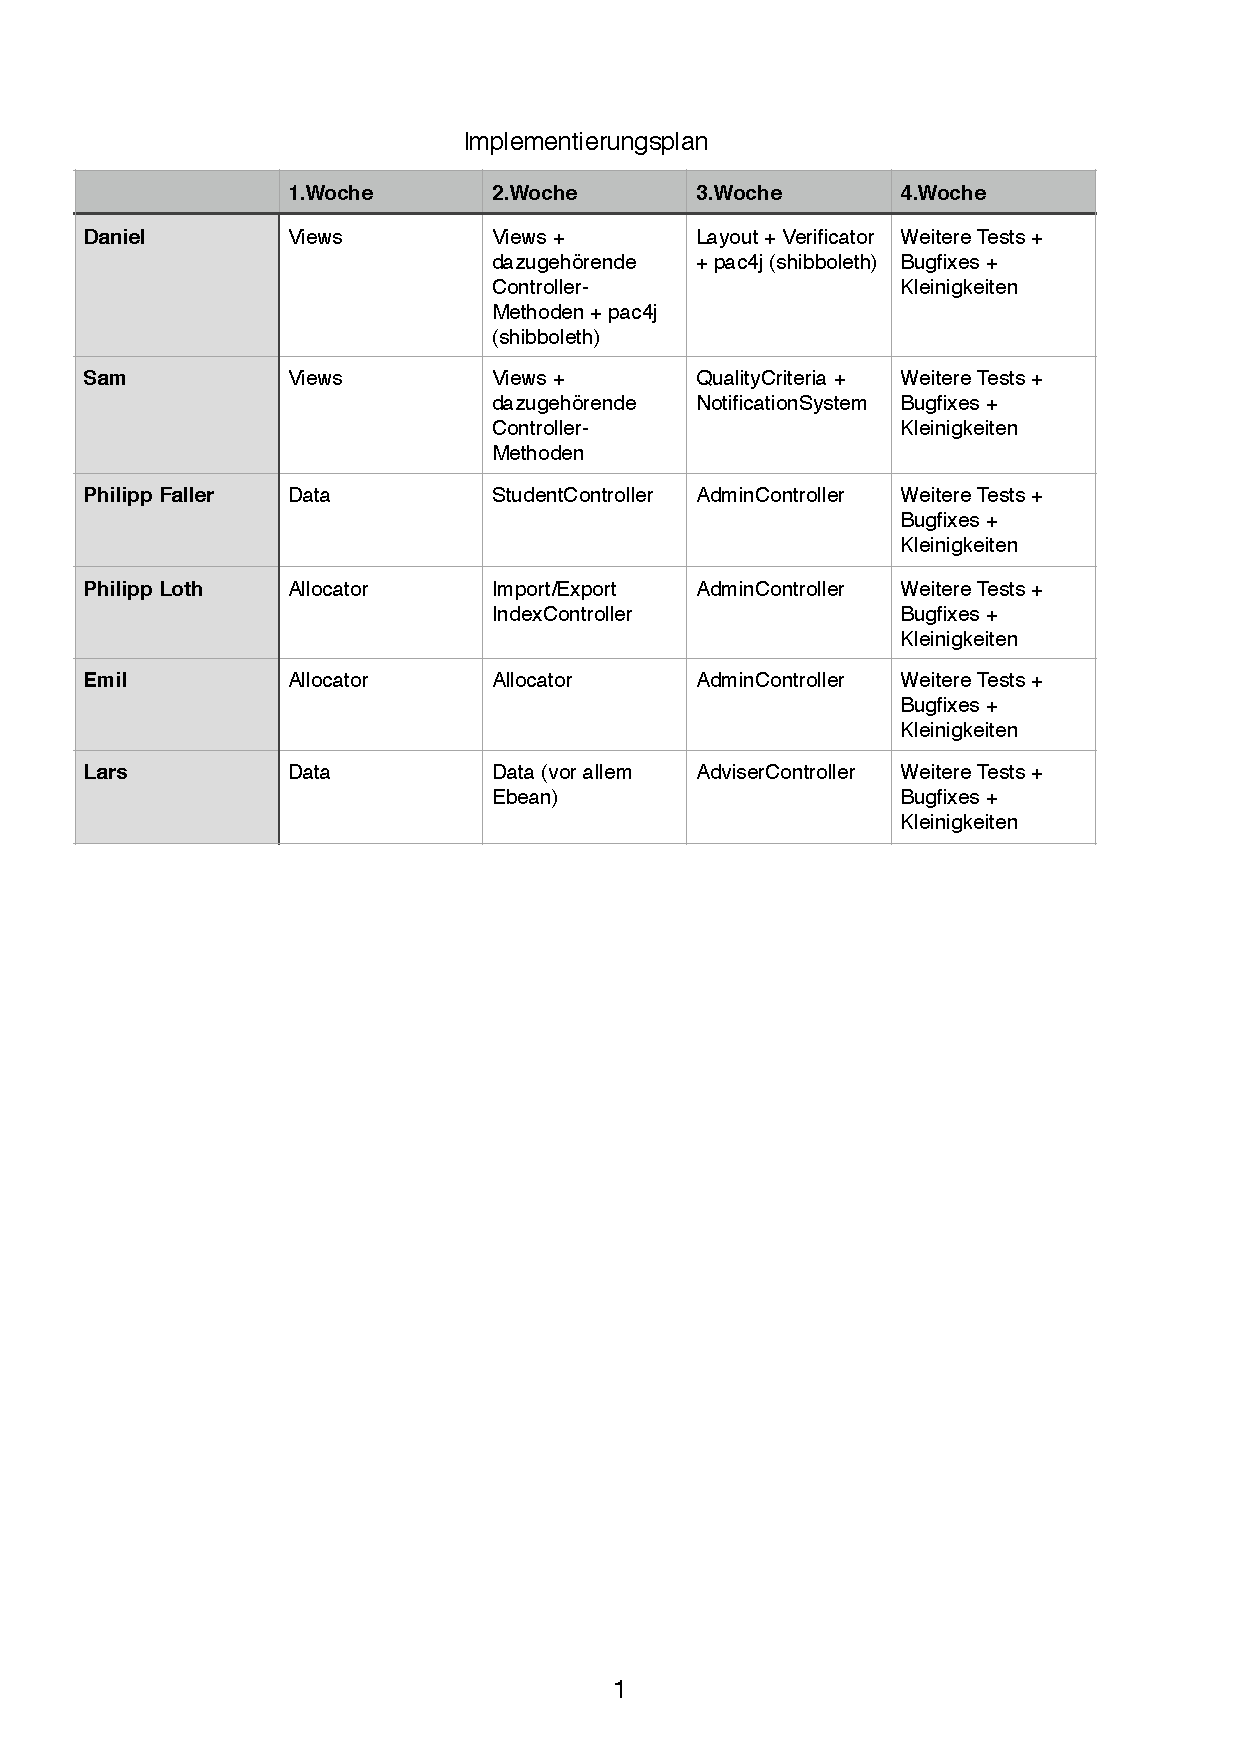
\includepdf[pages={1}]{Implementierungsplan.pdf}
Hierbei war der für uns \enquote{kritische Pfad} %TODO Was ist unser Criticall
% Path
%TODO zweites Diagramm wie haben wir wirklich implementeirt

%dann fairness bzw hierzu nur einen satz aber allgemeine statistiken 
%
\section{Änderungen zum Entwurfsdokument}
Zur Sicherung bessere Code-Qualität (z.B. dem Vermeiden von Code-Copy-Pasting)
und maßgeblich durch die oben beschriebenen Probleme mit verschiedenen
verwendeten Bibliotheken  wurden Änderungen im Vergleich zum  Entrurfsdokument
vorgenommen:
\begin{itemize}
  \item 
\end{itemize}

\section{Funktionsumfang}
Wie im Pflichtenheft beschrieben gibt es einige Muss und Wunschkriterien die 

%Muss und wunsch

%Tests

%Code Kommentieren nochmal?
\end{document}